
\section{SysMLv2 related decisions}

During this fifth deliverable we ran into the limitations pointed out in the fourth deliverable. In this section, we present these limitations. 


\subsection{Metadata feature library -- a promising idea}
\begin{figure}[ht] 
	\centering
	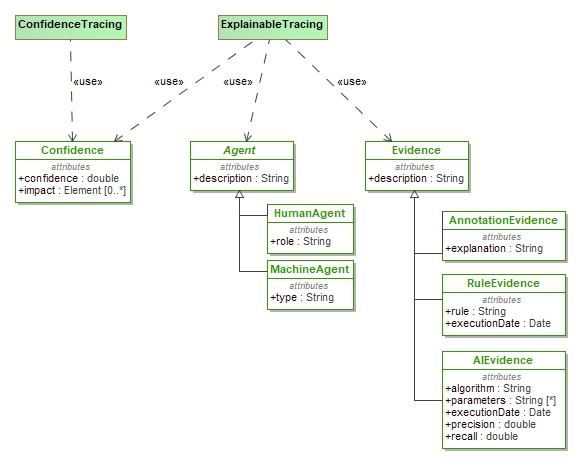
\includegraphics[width=.9\linewidth]{images/explainability-datatype.jpg}
	\caption{Metadatatypes for quality traceability including an assessment of confidence and monitoring of the identification processes used.}
	\label{fig:datatypes}
\end{figure}

% \vspace{3em}
The Listings \ref{lst:featurelibrary1} and \ref{lst:featurelibrary2} present our feature library {in SysML}. Listing~\ref{lst:featurelibrary1} contains the library declaration; Listing~\ref{lst:featurelibrary2} contains an example of application of such datatype  defined on a concrete example. It illustrates the allocation of a confidence value of 0.7 to a connection between a requirement (req) and a package. The second case (line 16 to 20) attributes a description and points to an element impacted (by the evaluation of the confidence),

% \vspace{10cm}

\begin{center}
\begin{lstlisting}[caption={Definition of a datatype dedicated to traceability (partial listing).},
label=lst:featurelibrary1,
style=mystylesysml,
linewidth=15cm,
xleftmargin=2.2cm,
morekeywords={part,filter}]
 package TracingAnnotations {
	attribute def ConfidenceTracing {
		attribute confidence : Real;
		attribute impact : Anything[*]
		assert constraint 
		  { confidence >= 0.0 && confidence <= 1.0 } 
	}
	 
	attribute def ExplainableTracing {
		attribute description : String;
		attribute evidence : Evidence;
		attribute agent : Agent;
	}  
 }
\end{lstlisting}
\end{center}  

\begin{center}
\begin{lstlisting}[caption={Use of metadata features for traceability},
label=lst:featurelibrary2,
style=mystylesysml,
frame=shadowbox,
rulesepcolor=\color{blue},
linewidth=15cm,
xleftmargin=2.2cm,
morekeywords={confidence,description,evidence,impact, part, req,package}]
 import package TracingAnnotations::*;

 /*Definition of the target system. */
 part vehiculetest {}
 req RE01_MLV {}
 package UMLCD_CORE {}

 /*Assignment of a confidence of 0.7 to the Req2Design link.*/
 connection Req2Design connect RE01_MLV to UMLCD_CORE {
   @ConfidenceTracing {
     confidence = 0.7;
   }
 }
 
 /*Assigning a description and an impact to the Req2Design link.*/
 connection Req2Design connect RE01_MLV to UMLCD_CORE {
   @ExplainableTracing {
     description = "Something";
     impact = (vehiculetest);
   }
 }
 
\end{lstlisting}
\end{center}


\subsection{Model level expression -- a deceitful implementation}
\begin{figure}[h]     
	\centering
	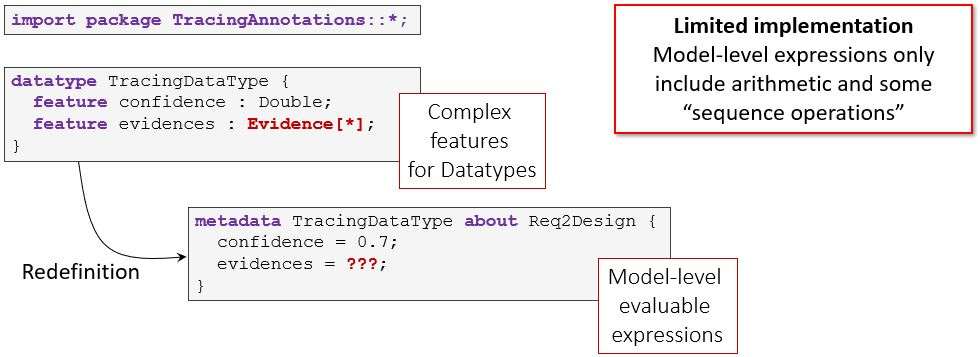
\includegraphics[width=.95\linewidth]{images/strategy4-metadatatype.jpg}
	\caption{Annotations and complex datatypes. }
	\label{fig:metadatatypes}
\end{figure}
When implementing these feature we ran into a number of disillusions. Fisrt and foremost, SysMLv2 implementation of the \textit{Model-level evaluable expressions} is for the least unsure. The concrete classes of the pilot implementation have been designed and written by only one developer (namely, Ed Seidewitz) and do not offer any safe guards. As showed in the previous deliverable, \Fig{fig:metadatatypes} points to where lies this limitation: when using a metadata feature, there is no guarantee for the use of "complex structures", \textit{i.e.,} that are not of basic types (int, double, String, ...). If used, these complex structure will at best show an error as pictured in \Fig{fig:filtererr}, and at worst keep the fallacious state of the system silent and leave the system out of its requirements.

\begin{figure}[ht]     
	\centering
	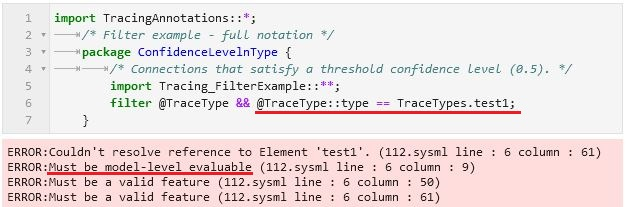
\includegraphics[width=.99\linewidth]{images/viz_filterexample_err.JPG}
	\caption{Limitation of the implementation of model-level evaluable expressions.}
	\label{fig:filtererr}
\end{figure}